\section{Glyph-based Solutions for Poetry Visualization}
\label{sec:poetry}

\subsection{Background}
Poems to some may be seen as nothing more than a sequence of words.
To poets however, they are a complex system with many links between words (\eg, rhyming patterns, and alliteration), different interpretations, and various ways of reading the same text (there is no indication of exact timing as in music for instance).
A technique called ``close reading'' aims to explore the complexity of such a system through hours of literary analysis devoted to a poem of interest. 
Such readings investigate many aspects of a poem including: 
\begin{enumerate}
	\item formal information (\eg, lines, and stanzas);
	\vspace{-2mm}
	\item phonetic information (\eg, meter, intonation, and timing);
	\vspace{-2mm}
	\item semantic information (\eg, genres, words, repetition, and sentiment); and
	\vspace{-2mm}
	\item context-driven information (\eg, geographical location, historical period, and political affiliation).
\end{enumerate}

\begin{figure}[b!]
\centering
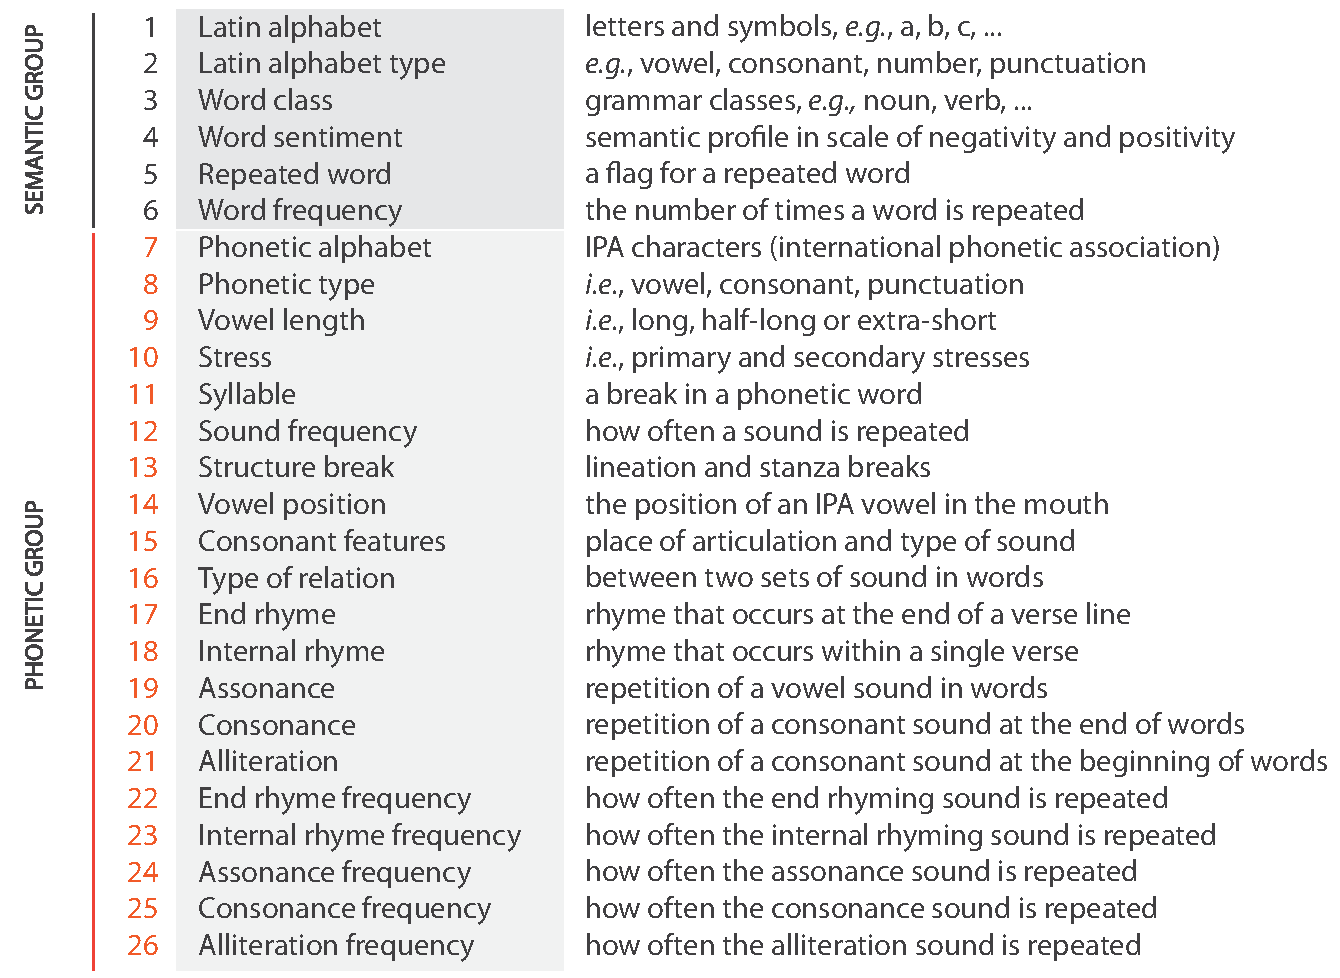
\includegraphics[width=\textwidth]{images/other_glyphs/poem_glyph_vars}
\caption{The six semantic and twenty phonetic variables representing a poem identified from investigatory discussions with domain experts.}
\label{fig:poem_glyph_vars}
\end{figure}


From investigatory discussions with the two poetry scholars from the University of Utah and a linguist from the University of Oxford, thirty-three variables were initially identified, although only twenty-six were deemed useful for poetry scholars.
These two set of variables shown in Figure \ref{fig:poem_glyph_vars} are there to help poetry scholars answer questions such as: 
\begin{enumerate}
	\item Which of the words in the poem rhyme with each other?
	\vspace{-2mm}
	\item What is the rhyming pattern in the poem?
	\vspace{-2mm}
	\item How much sound turbulence is in the poem (changes in the type of sound made through pronunciation of a word)?
	\vspace{-2mm}
	\item How many of the vowels are rounded vowels?
	\vspace{-2mm}
	\item Where are the caesurae (line pauses) in the poem?
	\vspace{-2mm}
	\item How many of the caesurae are masculine caesuras (pause following a stressed syllable)? and
	\vspace{-2mm}
	\item How many of the caesurae are feminine caesurae (pause following an unstressed syllable)?
\end{enumerate}

In all, fifty two tasks were identified.
Analysis of these tasks showed that not all variables were required all of the time. 
Classes of task required different variables.
What this meant in terms of visual design is that variables may have different levels of importance depending on the task at hand. 
This is in contrast to the work in the previous chapters where there was invariance in the importance of variables.

%The first piece of work investigates the use of knowledge from previous chapters to create a rule-based approach to help systematise glyph design. 
%Such a rule-based framework would allow for \emph{controlled} user-defined mappings of the twenty-six poem variables to visual channels.
The first piece of work investigates the creation of a visualization of poetry data facilitated by glyphs.
It also looks at the design of a mini-glyph required to show how sounds are produced in the mouth.

The second piece of work extends on the first through creation of static and animated overview glyphs (termed macro glyphs) for each line of a poem to show vowel sound changes/turbulence over time.
We use statistics to help creation of static and animated glyph designs.
This is followed by an evaluation of a selection of designs by four domain experts.

A web application named \emph{Poem Viewer} \url{http://www.ovii.org/PoemVis/} brings together both contributions for use by poetry scholars.

%although seven were removed due to not being suitable to English text (classification between pulmonic (sounds created by air-pressure from the lungs) or non-pulmonic consonants (ejective, implosive or click)), 

\subsection{Glyph Design for Poetry Visualization}

\subsubsection{Design Process}

Given the twenty six poetic variables defined in Figure \ref{fig:poem_glyph_vars}, the aim was to create a glyph design that would support their encoding and facilitate some fluidity in how the glyphs were constructed to support different types of task.
Our design process followed the ``nested model'' approach from Munzner \cite{munzner2009nested}.
This model was adopted due to its support for agile development with user engagement and inclusion of feedback at every stage of the design process.
Close interaction with domain experts was important in this work due to the poetry domain being relatively untouched by visualization research in the past.
Here we describe the design of the: 
\begin{enumerate}
\item \textbf{poem component glyph} that represents the features of each component, this being a word or punctuation mark for example in a poem.
Each glyph can connect to other glyphs to show relations between components of a poem (\eg, rhyming patterns and alliteration); and 
\item \textbf{vowel position ``mini glyph''} that shows the properties of vowel sounds and how they are produced.
\end{enumerate}

\textbf{Poem component glyph}. The overall glyph design needs to support encoding of the twenty-six poetic variables shown in Figure \ref{fig:poem_glyph_vars}.
The categorisation in Figure \ref{fig:poem_glyph_vars} divides the twenty-six variables in to semantic and phonetic groups.
Within each of these groups, further sub divisions can be made, these are:

\begin{enumerate}
\item\textbf{Phonetic}:
\begin{itemize}
\item \textbf{Phonetic Relations} between sounds and how they are pronounced \eg, rhyme, end rhyme (line endings that sound the same), alliteration, assonance (repeating vowel sounds), and consonance (repeating consonant sounds). 
%This region uses of line colour to represent the different types of relation, and line thickness to represent frequency;
\item \textbf{Phonetic Features} showing how the sound is made for vowels and/or consonants \eg, whether the sound is made from the back of the mouth with the tongue up (closed) or down (open) as shown in Figure \ref{fig:poem_glyph_design} B.
%This region makes use of pictograms like those shown in Figure \ref{fig:poem_glyph_design} B or symbol shape and colour to represent this data;
\item \textbf{Phonetic Units and Attributes} displays the phonetic alphabet, the type (vowel, consonant or punctuation), vowel length, stress (primary or secondary), syllable breaks, sound frequency, and structure break (new line);
\end{itemize}
\item\textbf{Semantic}:
\begin{itemize}
\item \textbf{Word Units and Attributes} displays the word, the type of each component within that word (vowel, consonant, or punctuation), the type of the word (\eg, noun, verb, adjective, adverb, or unknown), and the word sentiment; and
\item \textbf{Semantic Relations} between words of particular type or repetition of some word.
\end{itemize}
\end{enumerate}

A poem component can be a word or punctuation which may or may not have \emph{phonetic features}, \emph{phonetic units and attributes}, and \emph{word units and attributes}.
Each component can be linked together by their \emph{phonetic relations} (alliteration, assonance, consonance, or rhyme), or \emph{semantic relations} (repeated word, frequency, or sentiment).
Each poem component will be assigned a glyph representing it, alongside connections representing the relations between one or more poem components. 
This arrangement of glyphs creates the overall poem visualization.

Each of the sub divisions described above may be thought of as a region of the glyph.
These regions should be organised consistently to facilitate comparison between each glyph in a poem.
Furthermore, consistency will make it easier for users to perform visual search owing to the expectation of finding particular pieces of information in distinct areas of a glyph.
Two regions, \emph{phonetic relations}, and \emph{semantic relations}, require the representation of relational information.

\begin{figure}[b!]
\centering
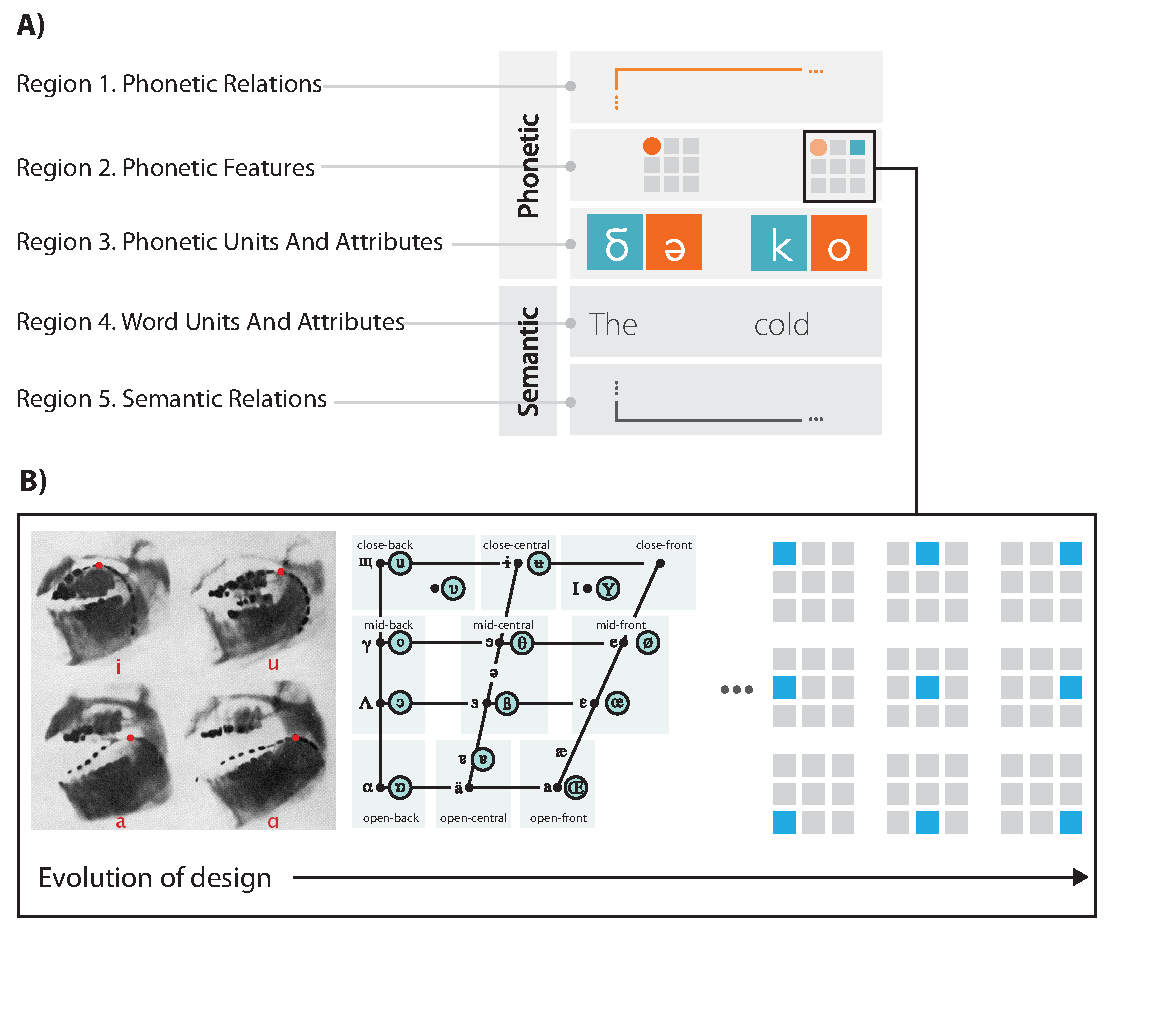
\includegraphics[width=.75\textwidth]{images/other_glyphs/poem_glyph_design}
\caption{A) The glyph design encompasses five regions to support semantic and phonetic variables listed in Figure \ref{fig:poem_glyph_vars}.
B) Evolution from the X-Ray scans of the mouth when pronouncing different vowel sounds, to the 5x7 IPA vowel chart, and finally to the 3x3 grid showing how the final sound is constructed by the different components of the mouth involved in speech.}
\label{fig:poem_glyph_design}
\end{figure}

The final arrangement of regions is shown in Figure \ref{fig:poem_glyph_design} and is largely driven by the phonetic/semantic divide.
Additionally, phonetic and semantic relation mappings were purposefully placed on opposite ends of the glyph to avoid line overlap. 
\emph{Phonetic units and attributes} were placed directly above the \emph{word units and attributes} since both were closely related and associating a word with a particular sound is important.
 
Due to users having changing needs, the type of data within some regions can be changed.
Additionally, the poetic to visual channel mappings can also be modified by users.
Appropriate mappings, or visual channels that are suitable for particular poetic variables, are automatically suggested to users via a ``rule-based mapping''  approach \cite{CGF:Abd2013a}.
This approach is inspired by the ``artificial assistant'' from Mackinlay \etal \cite{mackinlay2007show}, and informed by research presented in Chapters \ref{chap:related_work} and \ref{chap:glyph-tax}.


\begin{figure}[t!]
\centering
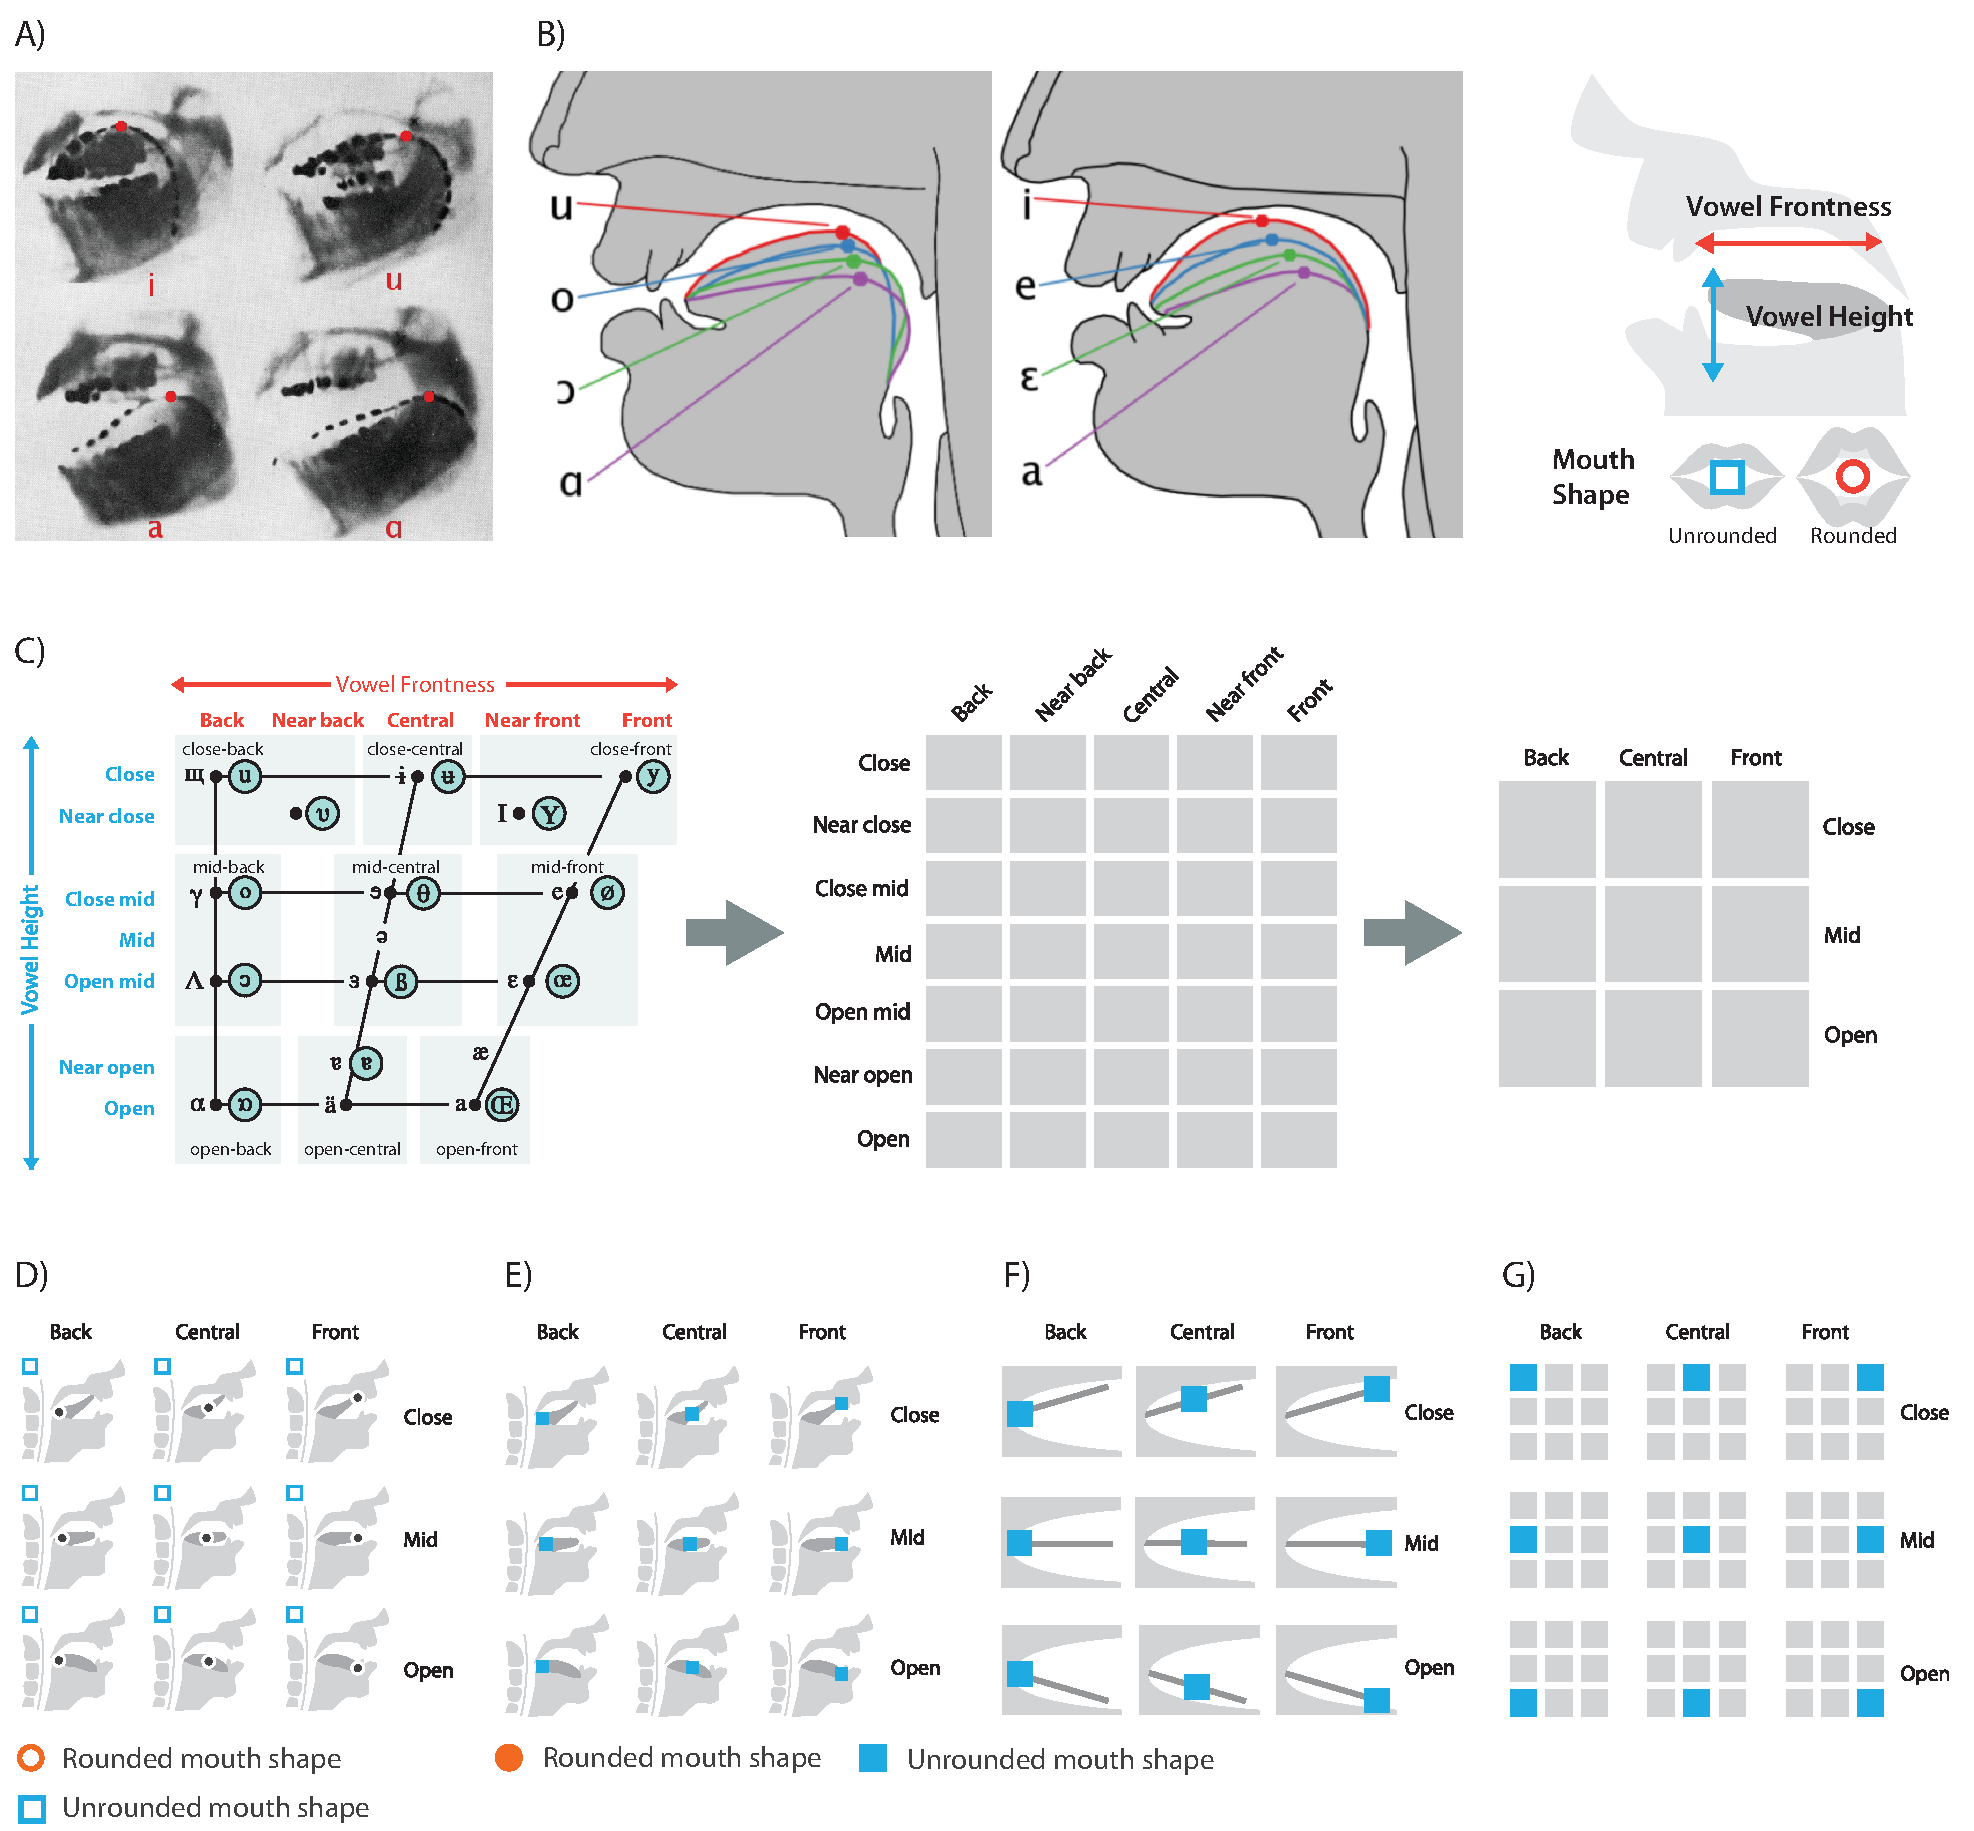
\includegraphics[width=\textwidth]{images/other_glyphs/poem-glyph-design-progression}
\caption{A) X-Ray scan from Jones \cite{jones1972outline} indicating the role of particular muscles in pronouncing certain vowels along with (some) marked up cross sections of a mouth and where vowel sounds originate.
Sound origin is shown with red marks that vary by height (vowel height) and distance from the back of the throat (vowel frontness).
B) Back (left) and front (right) vowel positions from Jones \cite{jones1972outline}.
C) The International Phonetic Alphabet (IPA) vowel chart \cite{ipa1999} arranges vowel sounds by the vowel height and vowel frontness properties that define those sounds in a 5x7 grid.
Through interactions with domain experts, it was found that this 5x7 matrix could be simplified to a 3x3 representation.
D) A first evolution of the design used a very metaphoric representation of the mouth, similar to those in \emph{B} and represent each of the positions from the 3x3 matrix achieved in \emph{C}.
The mouth is flipped since left was easier for users to interpret as the back due to how the glyphs were read from left to right.
Mouth shape is encoded by a shape in the top left of the mini glyph with a square with a blue stroke for unrounded, and an ellipse with an orange stroke for unrounded.
E) An extension of \emph{D} where mouth shape is encoded directly into the vowel frontness indicator as a square for unrounded and circle for rounded, with the addition of colour to provide further distinctiveness.
F) An abstraction on the first representation in \emph{C} that aimed to simplify the design for use in environments with lower resolutions. The line represents the tongue position.
G) The final 3x3 grid using coloured squares or circles at the position representing a vowel sound.}
\label{fig:poem_glyph_design_progression}
\end{figure}


\textbf{Vowel position ``mini glyph'' design}. In addition to the overall glyph design, a further design was devised to represent how a particular sound is constructed.
This ``mini glyph'', whose design process is summarised in Figure \ref{fig:poem_glyph_design} B, occupies the \emph{phonetic features} region in Figure \ref{fig:poem_glyph_design} A.
Each sound can be thought of as a particular configuration of specific muscles in the mouth.
This configuration includes the tongue position (vowel height), the shape of the mouth (rounded or unrounded), and the location in the mouth a particular sound originated (vowel frontness).
Figure \ref{fig:poem_glyph_design_progression} A shows a cross section of a mouth along with the different tongue positions (vowel height) and where in the mouth a sound originated using a red dot (vowel frontness).
Figure \ref{fig:poem_glyph_design_progression} B shows an abstract view of different vowel sounds and the configurations of vowel height and frontness that make these sounds possible.

The remaining components of Figure \ref{fig:poem_glyph_design_progression} show how the final glyph design came about and the design iterations made in chronological order from the initial abstraction step in Figure \ref{fig:poem_glyph_design_progression} C to each of the design options shown in Figure \ref{fig:poem_glyph_design_progression} D - G.
Figure \ref{fig:poem_glyph_design_progression} C starts with the IPA vowel chart \cite{ipa1999} that provides an organisation of the different vowel sounds by their vowel height and frontness parameters.
The chart may be represented by a 5x7 matrix, however this would be sparse since not all thirty-five positions would be used.
Following interactions with the domain experts, it was advised that this could be simplified to a 3x3 representation.

This 3x3 grid provided the general configurations of vowel height and frontness that needed to be represented by the mini glyph.
Further design iterations from Figure \ref{fig:poem_glyph_design_progression} D to G investigated the numerous ways glyphs could be represent to represent each configuration. 
Figure \ref{fig:poem_glyph_design_progression} D started with the mouth representation seen in Figure \ref{fig:poem_glyph_design_progression} B.
The hope was that a more metaphoric representation would make it easier for users to identify where sounds were coming from.
The tongue angle varies to reflect vowel height.
The position of the ellipse on the tongue represents the vowel frontness.
Progressing from this design, Figure \ref{fig:poem_glyph_design_progression} E encoded mouth shape directly on the vowel frontness indicator, using colour to provide increased differentiability.
Although the domain experts liked the design, the glyphs were difficult to interpret at lower resolutions, therefore we devised the design in Figure \ref{fig:poem_glyph_design_progression} F.
This kept the mouth metaphor in place, but made it more abstract so that more space could be afforded to the visual elements encoding information.
Again, users sometimes found it difficult to see differences between glyphs at the lower resolutions.
The final design, shown in Figure \ref{fig:poem_glyph_design_progression} G is able to represent all possible states through just using position, with colour and shape representing the mouth shape.
This design, although less metaphoric than the mouth could be interpreted even when the glyph was very small, so users preferred it.

\begin{figure}[t!]
\centering
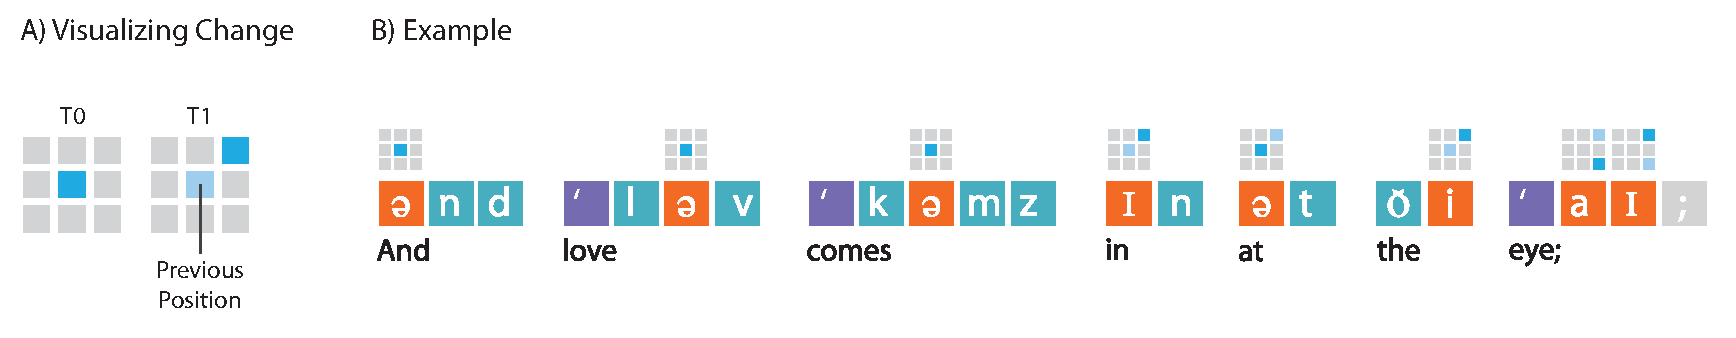
\includegraphics[width=\textwidth]{images/other_glyphs/poem_glyph_change}
\caption{A) The previous sound is maintained through making the shape representing that sound more transparent. B) In this poem, the changes can be seen in mouth position with the main sound being a front closed position (top right square) with an unrounded mouth.}
\label{fig:poem_glyph_change}
\end{figure}

Additionally, as shown in Figure \ref{fig:poem_glyph_change}, information about the previously encountered sound can be added to the glyph.
Showing the previous state allows users to see changes in the sound dynamics.
Smooth passages of sound should have relatively small changes, conversely, rough passages will have a greater number of changes.

\subsubsection{Evaluation}
The evaluation and design process were very much entwined in this work with frequent testing and feedback from domain experts that were part of a remote collaboration with poets from the University of Utah (Prof. Katherine Coles and Dr. Julie LeIn).


\subsection{Macro Glyphs for Poem Turbulence Summaries}

Following the initial poem glyph design, the poets wished to be able to gain an overview of how the sounds within a poem evolve/flow over time, a property known as the ``poem turbulence''.
From the previous work that presented a pictorial glyph design, it was not easy to follow the changes in sound over time.
The poetry scholars wished to observe patterns in sound changes to determine if certain types of poems have a particular type of ``turbulence pattern'', or within a poem are there patterns in sounds between lines?

While the first glyph design process used the nested model by Munzner \cite{munzner2009nested} as a framework to follow, this work followed a computational approach to glyph design as outlined in Chapter \ref{chap:strategies} with a user evaluation at the end.
In terms of process, this translates into the use of computational approaches to inform the design. Contrast this with the first piece of work where we relied heavily on user engagement to reach a final design.

\subsubsection{Macro Glyph Design Process}

Similar to Chapter \ref{chap:automacron}, this work proposes the use of ``macros'' (overview representations) to assemble many sound transitions in a single glyph.
This approach would solve the issue experienced by poets who wish to be able to see the overall flow of sounds across a line or poem as opposed to reading each pictogram for a vowel or consonant sound one by one.  
However, multiple macro design solutions are possible, all with advantages and disadvantages.
For this type of task, flow can be shown either statically or dynamically.
In this work we investigate a number of design options, both static and dynamic created using many of the techniques presented in the previous chapters to aid more systematised glyph design. 
The design options are evaluated with a number of poetry scholars to determine which performed better for tasks involved in understanding the sound patterns in poems.  

Of particular relevance to this thesis is the statistical approach taken in the design of the glyphs.
Thirty-five poems and other English texts (books and scientific publications) were analysed to determine the sounds and transitions present in the English language.
By analysing not just poems, a more accurate view of the transitions that occur in spoken English can be obtained.

\begin{figure}[t!]
\centering
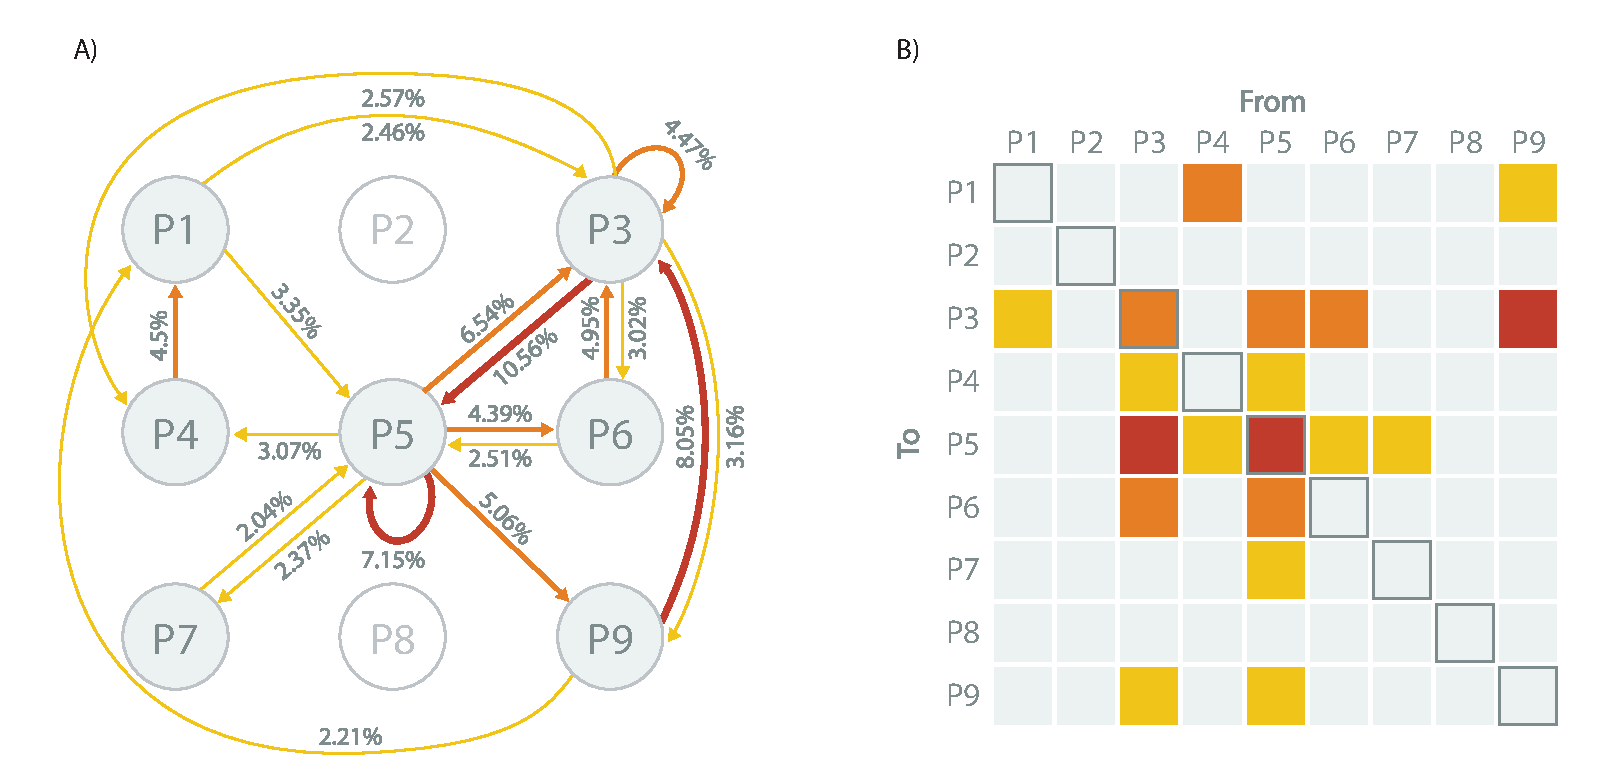
\includegraphics[width=\textwidth]{images/other_glyphs/macro_stats}
\caption{A) Graph showing vowel positions (see Figure \ref{fig:poem_glyph_design_progression} G) using nodes and the movements between each position using weighted edges as found in an analysis of 30 poems and English text.
The network shows that two positions are not used in the corpus of data observed.
B) Heat map showing the active areas in the network. 
Both A) and B) are coloured by the number of transitions from one position to another (grey is $f(p_a, p_b) = 0\%$, yellow ($0\%<f(p_a, p_b)< 4\%$), orange ($4\%<=f(p_a, p_b)<7\%$), and red ($f(p_a, p_b)>=7\%$)) where $p_a$ is the \emph{from} position and $p_b$ is the \emph{to} position.}
\label{fig:poem_statistics}
\end{figure}

The statistics gave us answers to the following questions: 
\begin{enumerate}
\item \emph{How many vowel phonemes (sounds that make words sound different from each other) were there per line?} The analysis showed that 84.3\% of lines contain $\leq$12 vowel phonemes and 22 is the maximum number of vowel phonemes;
\item \emph{How many movements were there in the frontness of the sound (back to front)?} The average difference in movement in movement is $\bar\mu=0.7709$ and the standard deviation $\sigma=0.7073$;
\item \emph{How many movements are there between open and closed tongue positions (termed vowel frontness)?} The average difference in movement in movement is $\bar\mu=0.8704$ and the standard deviation $\sigma=0.6699$; and 
\item How many transitions occurred between each position? The results to this are shown in Figure \ref{fig:poem_statistics}.
\end{enumerate}

The \textbf{static radial macro glyph} design benefitted from statistics 1) to 3). 
When the design process started, the number of spokes or lines representing each vowel phoneme was unknown. 
The seemingly obvious idea to make the number of lines dynamic would in fact make comparison between lines and positions more difficult. 
A small number of lines may result in the need for many macro glyphs to represent a line.
Conversely, a large number would result in a very densely packed macro glyph that was difficult to visually parse.

Statistic 1) showed that 84.3\% of lines contained twelve vowel phonemes or less, while the maximum number of vowel phonemes was twenty-two. 
Twelve fits well with the clock metaphor, and since the temporal aspect is important, familiarity with the clock would make such a glyph easier to interpret. 
The 15.7\% of lines that have more than twelve vowel phonemes would be accommodated through the use of two macro glyphs side by side. 
Alternatively, a twenty-four line glyph that could also fit the clock metaphor, could represent all of the vowel phonemes in lines, however 84.7\% of those lines would occupy less than half of the area of the glyph, and the more densely packed macro glyph would likely be more difficult to interpret.

Statistics 2) and 3) were used to inform which axis of the 3x3 vowel sound matrix (vowel frontness and height) would be mapped to a suitable visual channel. 
The variable with the greatest difference and deviation would be the ideal candidate for a mapping to position.
Unfortunately there was no outright winner, with vowel frontness having the larger standard deviation and vowel height having the largest average difference.
This led to a decision that proposed both options for evaluation by poets themselves to determine which mapping was more effective.
 
The \textbf{animated macro glyph} benefitted most from statistic 4). 
This statistic, summarised in Figures \ref{fig:poem_statistics} A and B, shows how many transitions there are between across the 3x3 matrix. 
Figure \ref{fig:poem_statistics} A shows a graph depicting all observed transitions with their probability of occurring.
Figure \ref{fig:poem_statistics} B presents a matrix-based representation of the graph view. 
It clearly indicates how only a small subset of all possible transitions between sounds are observed in the data (19/81), that positions two and eight have no observed uses, and finally that the greatest activity occurs around positions three and five.
Such analysis of the data would indicate that we can:
\begin{enumerate}

\item \emph{inform} the design process and implementation of the glyphs by exposing what transitions do and do not happen (from this analysis 19/81 transitions are observed in the data).
Therefore, instead of creating a glyph that needs to represent all possible transitions between nodes in the graph, many of these hypothetical transitions may be ignored, greatly simplifying the glyph design; and

\item enable the \emph{highlighting} of rare transitions and/or playing down the significance of frequent transitions if poets desired such functionality.

\end{enumerate}

The ability to inform the design process thanks to statistical analysis greatly simplified the design of the glyphs since the arcs between each position could be better arranged and decluttered.
For example, the knowledge of absence of transitions to/from positions two and eight made it possible to inform the animation algorithm to decrease the height of arcs running through positions one and three, and seven and nine. 
Additionally, where connections were uni-directional, the arcs could be less curved than they need to be when visualising a bi-directional connection. 

\begin{figure}[t!]
\centering
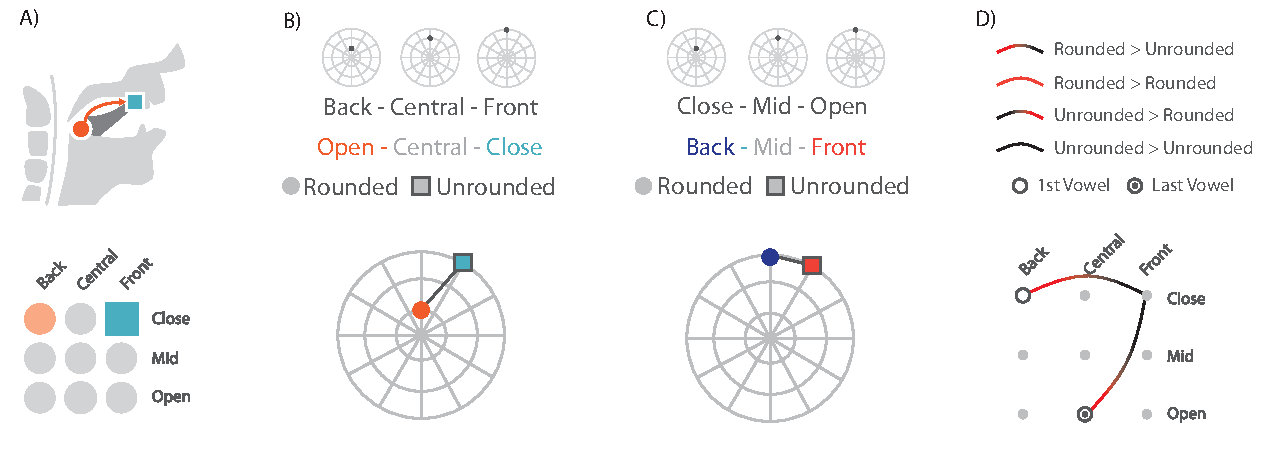
\includegraphics[width=\textwidth]{images/other_glyphs/poem_macro_design}
\caption{Four glyph representations showing how a particular sound is formed.
A) This is the original representation of sound movement.
B) A radial layout where time zero is at the top. This representation supports eleven sounds arranged temporally where the difference in distance from the inner to outer rings indicates the change in the sound origin (back to the front of the mouth).
C) An alternative radial layout where the position relates to the tongue being opened, in the middle, or closed.
D) An animated glyph design showing the flow between points in the 3x3 matrix using animation.
}
\label{fig:macro_glyph}
\end{figure}

Figure \ref{fig:macro_glyph} shows the resulting designs of the static radial macro glyphs and the overall schematic for the animated macro glyphs.
 

\begin{figure}[t!]
\centering
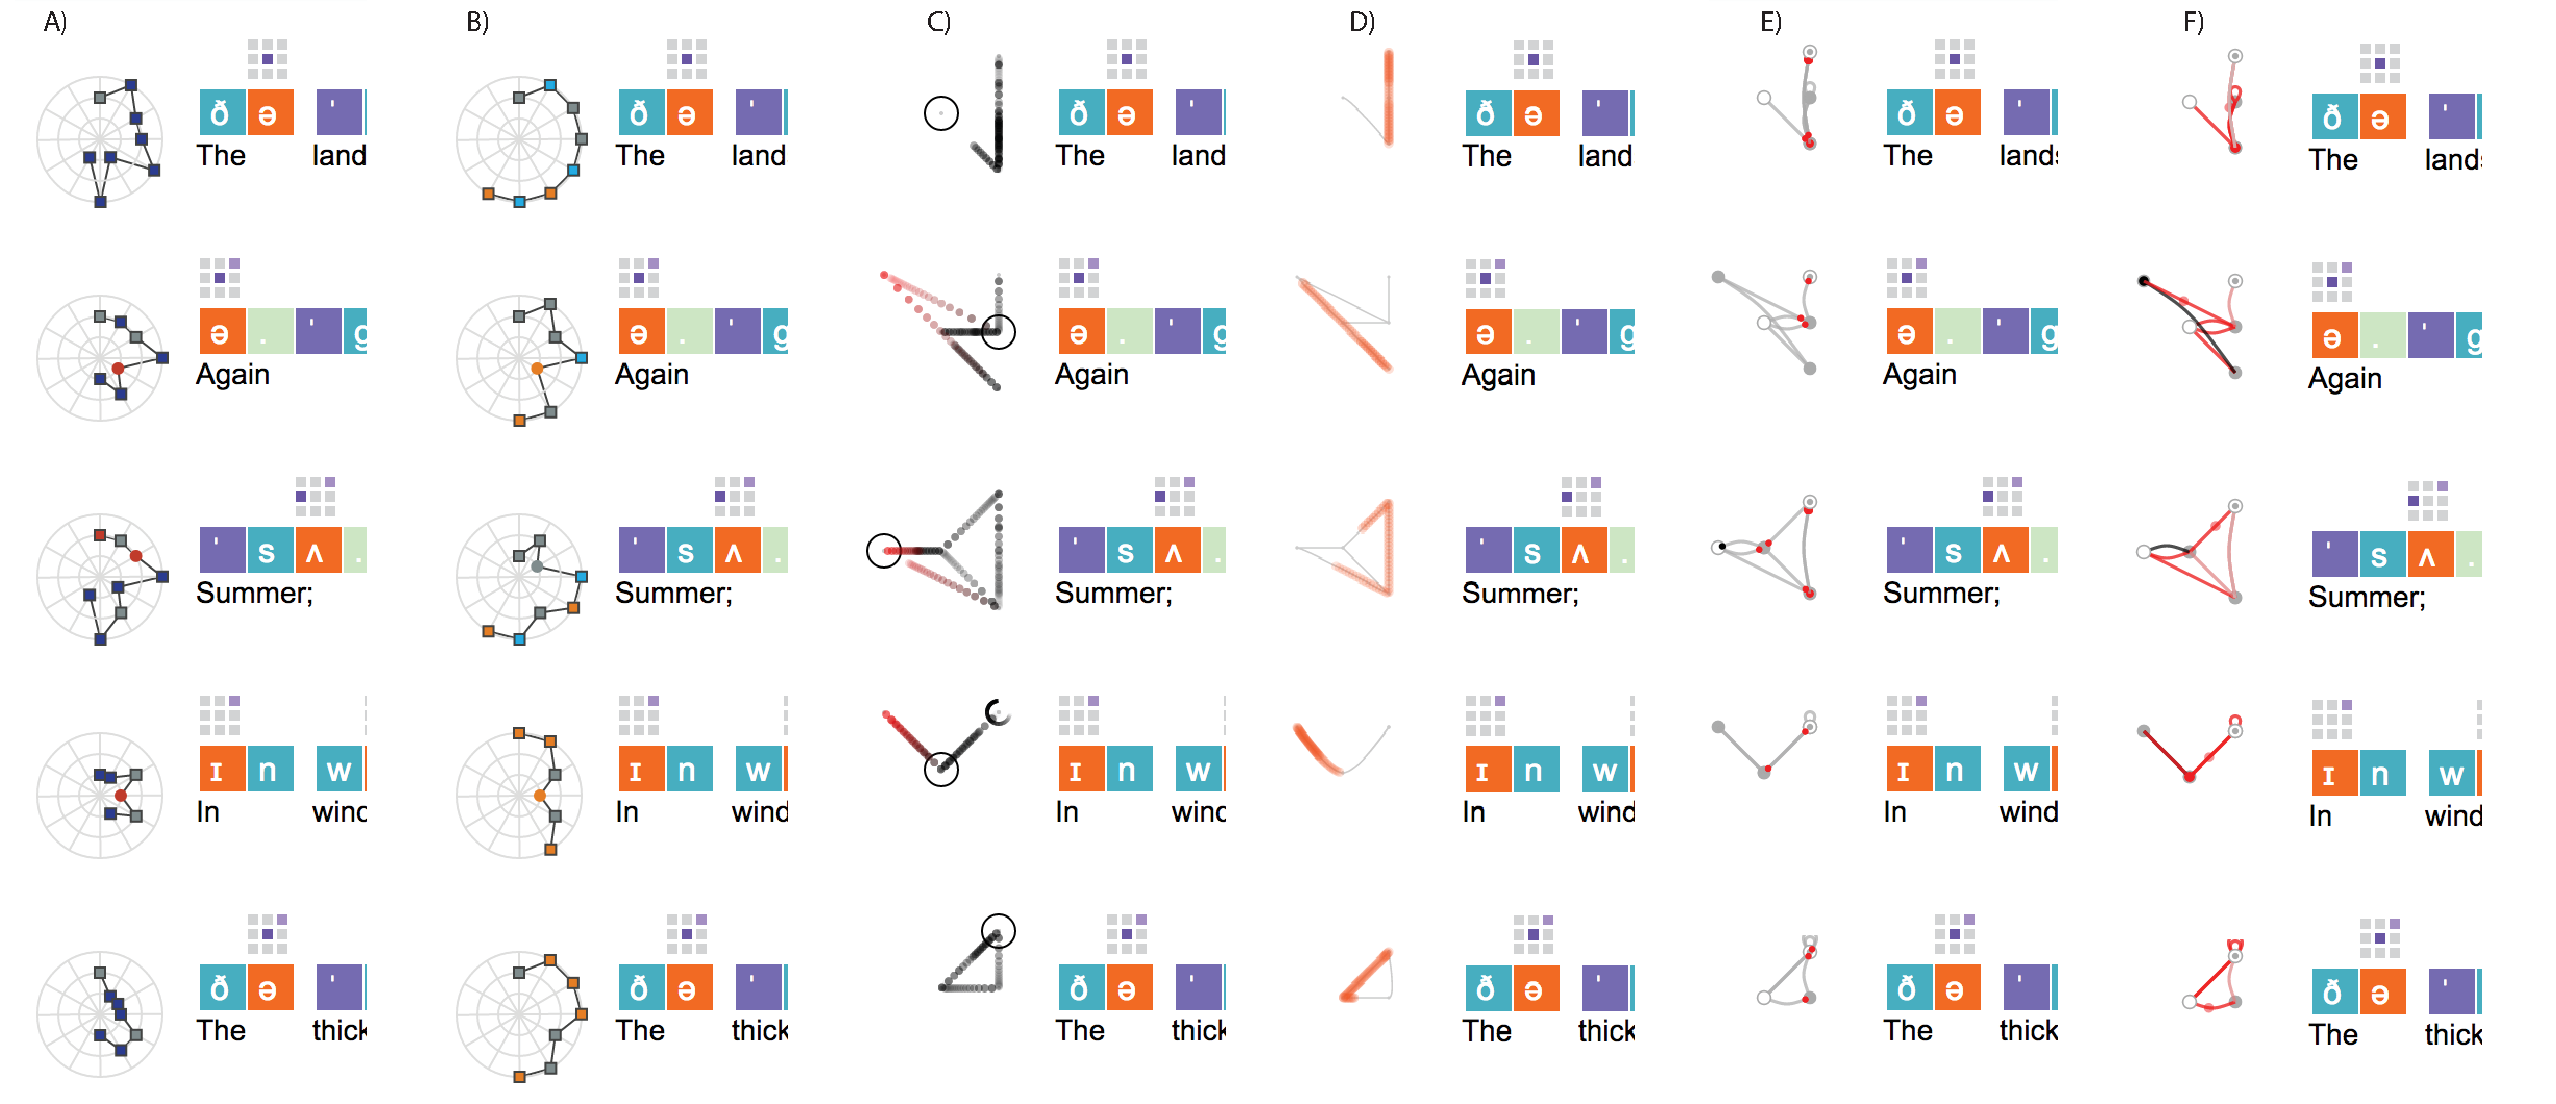
\includegraphics[width=\textwidth]{images/other_glyphs/macros_options}
\caption{Six macro glyphs visualizing five lines of the same poem. 
A) Static radial layout with radial position representing back to front of the mouth.
B) Static radial layout with radial position representing close and open positions of the tongue.
C)-D) Animated transition macro glyphs with trails highlighting previous position. 
E)-F) Animated transition macro glyphs with markers and permanent trails highlighting previous positions.
A video showing the animated glyphs can be found at \url{https://vimeo.com/120620233}.
}
\label{fig:macro_glyph_implementation}
\end{figure}

Figure \ref{fig:macro_glyph_implementation} presents the implementation of the two static macro glyphs, and four variations of the animated macro-glyph, used to visualise five lines of the same poem. 
Due to an understanding that animated glyphs may prove difficult for users wishing to preserve previous transitions, a number of animations were attempted.
Figures \ref{fig:macro_glyph_implementation} C to F represent these different animation strategies to be assessed by expert users.

\subsubsection{Evaluation}

To evaluate the effectiveness of the macro glyph representation, three postgraduate students in English and French literature, and a Professor of Italian literature were invited to an evaluation session. 
The evaluation consisted of a demonstration of the three designs and the variations of the animated glyphs shown in Figure \ref{fig:macro_glyph_implementation}, followed by a questionnaire consisting of forty-three questions, a discussion, and finally an opportunity to change answers based on the discussions and answers they received.

The responses are summarised as follows:
\begin{itemize}
\item \textbf{Static Radial Macro Glyphs}
\vspace{-1mm}
\begin{enumerate}
\item Both types of radial representations are important to scholars depending on the task;
\vspace{-2mm}
\item Helpful in: a) identification of phonetic patterns among lines; and b) differentiation of dynamics and structures in poems;
\vspace{-2mm}
\item Circles and squares work well for differentiating between rounded and unrounded vowels respectively; and
\vspace{-2mm}
\item The logo logical link between the colours used and say open (orange) or closed (cyan) tongue made remembering the colour coding an easier process.
\end{enumerate}
\vspace{-2mm}
\item \textbf{Animated Transitions}
\vspace{-1mm}
\begin{enumerate}
\item Entertaining to watch;
\vspace{-2mm}
\item Intuitive to use when observing the general flow but after some time, the temporal ordering is lost; and
\vspace{-2mm}
\item Opacity as a tool for encoding frequencies is helpful but it can present ambiguity;
\end{enumerate}
\vspace{-2mm}
\item \textbf{Static Transitions with Temporal Highlight}
\vspace{-1mm}
\begin{enumerate}
\vspace{-2mm}
\item Similar to the \emph{Animated Transitions}, it is intuitive, but the ability to track is lost after some observation time;
\vspace{-2mm}
\item Residual line patterns show direction and frequency well, but temporal ordering is not shown; and
\vspace{-2mm}
\item The moving highlight is helpful but not enough to enable the remembering of temporal ordering.
\vspace{-2mm}
\end{enumerate}
\end{itemize}

Although the animated macro glyphs were entertaining for users and did contribute to the analysis of the poem, the most useful macro glyphs for determining the relations between lines of poems were the static representations.
The issues with animation were understood in advance of this work, in particular the problems with depicting temporal information.
However, they still proved useful for depicting overall flow of information. 

\subsection{Poem Viewer}

\begin{figure}[t!]
\centering
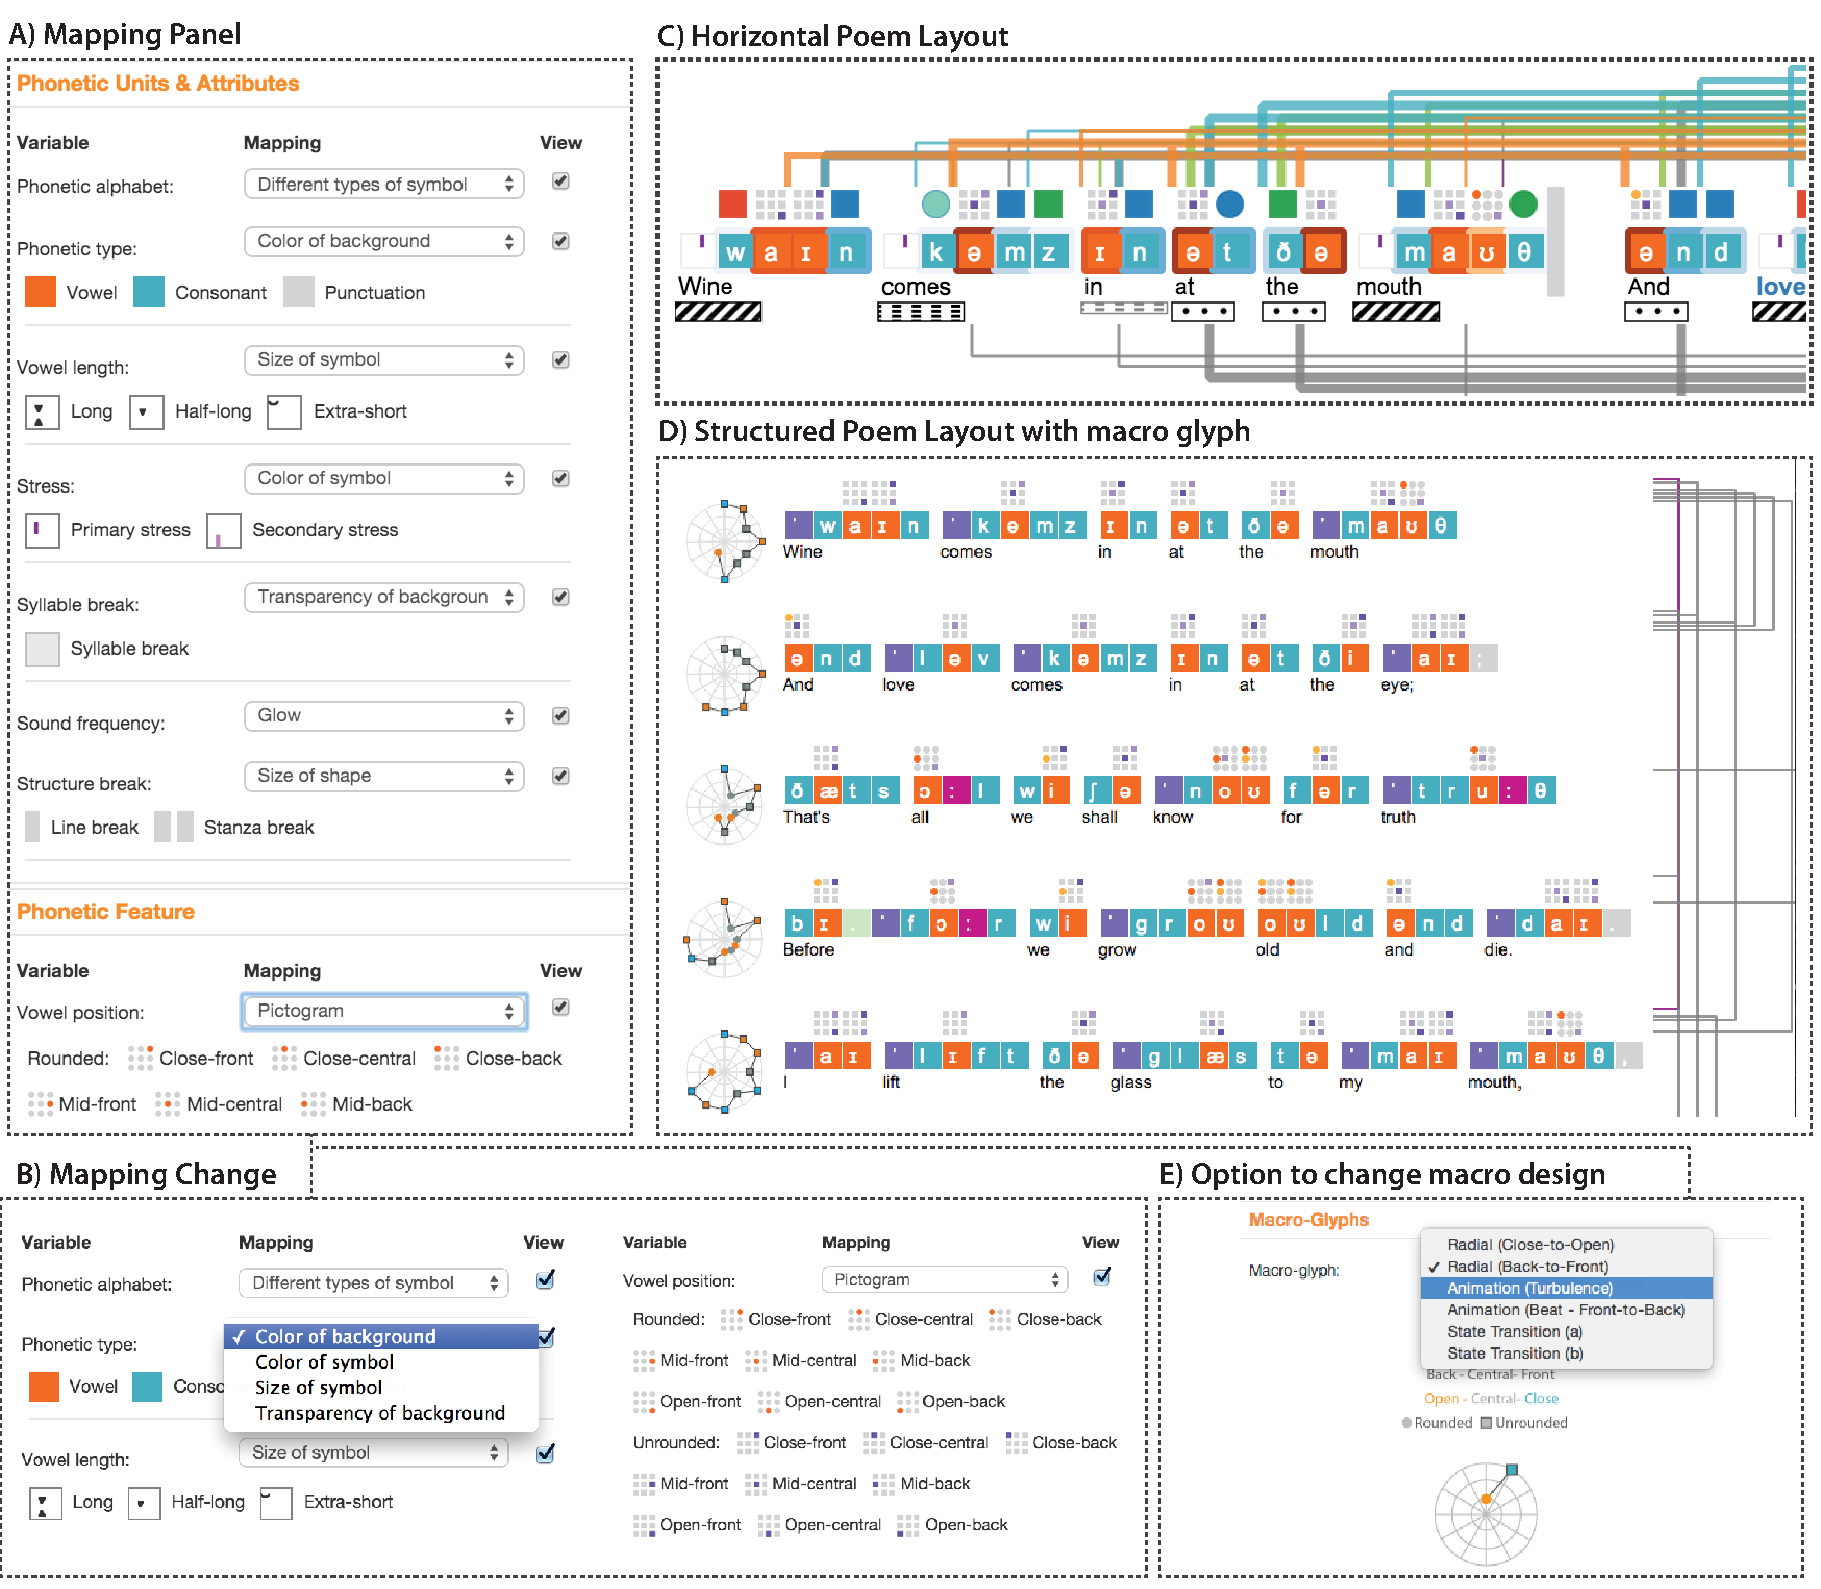
\includegraphics[width=\textwidth]{images/other_glyphs/poemview_overview}
\caption{The Poem Viewer interface.
A) The mapping panel allows users to specify how poem variables are mapped to visual channels.
B) Some examples showing mapping restrictions devised from the rule-based approach.
C) The poem can be viewed horizontally or in its structured layout in D) which also shows the macro glyphs for poem turbulence.
E) A number of macro glyphs, static and animated can be used to visualize the data.}
\label{fig:poem_view_overview}
\end{figure}


Both pieces of work were integrated in PoemViewer \url{http://www.ovii.org/PoemVis/} shown in Figure \ref{fig:poem_view_overview}, an online tool that supports poem upload and visualization functionalities.
Additionally, the interface supports ``rule-based mappings'' so that users can configure visual mappings from poetic variables in a controlled way. 

